\chapter{Controlling overproduction}
\todo{still not happy with this title}
\label{chap:exploring-the-problem-space}
In the previous chapter we established the definition of a \textit{reactive program} in terms of its behavior, how it is implemented in Rx, what the danger is of having an overproducing \obs and which solutions already exist to solve this problem. In this chapter we will discuss these solutions in further detail, consider their advantages and disadvantages and argue which solutions work for the various kinds of streams. Based on this discussion we will propose a new approach for controlling the flow of an overproducing \obs.

\section{Hot and cold streams}
Applying the definition of reactiveness by Benveniste and Berry \cite{berry1991-Reactive} to the Rx \obs, we can conclude that every \obs sequence starts with a source that emits values at its own pace. No matter which function is used for this (\code{apply}, \code{range}, \code{timer}, \code{interval}, etc.), ultimately they all are the result of the \code{Observable.create} function. This function lifts an arbitrary source into the \obs interface and treats its values like streaming data. The behavior that is exposed by the resulting stream can however differ from source to source.

Sources like clocks, mouse moves or key presses start emitting whenever it desires, regardless of any \obv being subscribed to the stream. When no one is listening, the data is simply discarded; when multiple \obv instances are subscribed, every one of them receives the same data at (approximately) the same time. In case an \obv subscribes on a later moment, it will not receive all previously emitted data, but will only share in the data that is send after it is subscribed. This kind of source is considered to be \textit{hot}. It is strictly reactive, meaning that it can only emit data at a speed which is determined by the source and has no way to be slowed down by any \obv that cannot cope with the amount of data sent.

On the other hand there are streams that originate from sources that are actually interactive. These include the results of database queries and \ieb sequences. Often the reason for them being wrapped into an \obs is because of a potential delay that needs to be awaited before the result is returned, without blocking the program flow or call stack. It may, for example in case of lazy evaluation, take some time before the \ier has produced its next element. The \obs will however not start emitting its data immediately, like the hot variant, but will wait until at least one \obv is subscribed. Only then it will start producing its values. In case a second \obv subscribes, the stream will effectively duplicate itself and start all over again with emitting the first values. Unless specified by operator sequences, this means that the lazy \ier in the source will have to produce its values a second time as well. In the end, both the first and second \obv have received the same set of data, even though the second subscribed much later than the first. A stream with this kind of behavior is referred to as a \textit{cold} \obs.

In the rest of this chapter we will distinguish between two types of the cold \obs. First there is the \textit{cold with-latency \obs}, which is bound by a certain notion of time. This type wraps a source that is interactive, but can take some time before it produces its next element. Examples of this can be a network response, the result of a database query or an \ieb sequence where each element is computed lazily and therefore takes some time to be returned. On the other hand we distinguish the \textit{cold no-latency \obs}, which is \emph{not} bound to any notion of time. This type mainly wraps interactive sources for which the values are already computed, such as a list.

In short, a hot \obs has a source that is strictly reactive, whereas a cold \obs originates from a source that is interactive. With the latter, an \obv could potentially ask the \obs to slow down by generating elements less frequently, even though this would strictly speaking be against the definition of reactiveness. The \obs would not have to buffer unbounded amounts of elements that cannot be consumed immediately, it will just generate its elements in a slower pace.

This is however not possible for a hot \obs, since it reacts to events from the outside environment. It is not possible for an \obv to ask the source to slow down the movement of the mouse, nor is it possible for the \obv to request less frequent key presses or clock ticks. These events are dependent on a notion of time; their speed is determined by the environment \cite{berry1991-Reactive}.


\section{Solutions for overproducing sources discussed}
In the previous chapter we described an interesting problem that occurs when working with streaming data and reactive programming: ``\textit{what happens when the consumer cannot handle the data flow presented by the producer?}''. We also presented a number of solutions, ranging from putting data in an overflow buffer to gaining more control over the \obs. Some of these solutions work perfect under certain conditions, others do not. In this section we will discuss the solutions that were described in section~\ref{sec:fastproc-slowcons} in further detail and reflect on them in the light of the previous section on hot and cold streams.

\subsection{Avoiding overproduction}
As described in section~\ref{subsec:avoiding-overproduction}, \textit{avoiding} is a first line of defense for overproduction. This was done by introducing several operators that either drop some of the data or buffer the data and propagating these buffers downstream for further manipulation. All lossy operators, as well as the \code{buffer} with interval, require a \sch for them to run their interval timers on, hence the output stream of these operators runs on a different thread.

For a hot \obs this kind of defense mechanism is perfect, as the speed at which the source is producing is unknown. This also holds for the cold with-latency \obs, as the production of elements is also bound to a notion of time. For other cold streams, like \code{Observable(1, 2, 3, 4)} or an \obs that is created from a list of elements as shown in \autoref{lst:obs-from-seq}, it does not make any sense to add any overproduction-avoiding operators, as this kind of stream is sequential and will in fact emit at a rate which is determined by the \obv.

\begin{minipage}{\linewidth}
\begin{lstlisting}[style=ScalaStyle, caption={Observable from \code{Seq[T]}}, label={lst:obs-from-seq}]
def fromSeq[T](list: Seq[T]): Observable[T] $=$ {
    Observable.create(observer $\Rightarrow$ {
        list.foreach(observer.onNext)
        observer.onCompleted()
    })
}
\end{lstlisting}
\end{minipage}

We are aware of the fact that these operators also have use cases other than avoiding overproduction, such as edge detection or calculating the derivative of a stream of numbers. However, these use cases fall outside the scope of this thesis and for them the comments above do not apply.

\subsection{Callstack blocking}
Subscribing to an \obs is basically nothing more than supplying an \obv to the function within \code{Observable.create} and \emph{sequentially} executing this function using this provided \obv. Once an element is emitted by the source, all operations in the \obs sequence are executed on that element before a second element is emitted. In the sequence of operators in \autoref{lst:operators-obs}, first all operations on $1$ are performed, before $2$ is emitted by the \obs (and then discarded by \code{filter}). This is also the case in \autoref{lst:observeOn} up to line~\ref{line:observeOn-in-observeOn}, after which the elements are scheduled on a different thread and hence are further processed in parallel with emitting new elements from the source.

The order of operations is designed this way to allow for lazy evaluation: never run code that does not need to be run. If a cold \obs contains 5 elements and the operator sequence contains the operator \code{take(2)} (see \autoref{lst:lazy}), only the first 2 elements from this \obs will be evaluated, rather than all 5. After the second element has passed \code{take}, it sends an \code{onCompleted()} downstream, right after the second \code{onNext}, causing the stream to end without evaluating the other 3 elements.

\begin{minipage}{\linewidth}
\begin{lstlisting}[style=ScalaStyle, caption={Lazy evaluation}, label={lst:lazy}]
Observable(1, 2, 3, 4, 5)
    // some operators
    .take(2)
    // some more operators
    .subscribe(i $\Rightarrow$ print(i + " ")) // only prints the first and second element
\end{lstlisting}
\end{minipage}

Following this order of operations, we can conclude that basically every higher order function that is executed in the operator sequence is in a sense blocking the callstack during its computation and thereby preventing the source from emitting a next element until the previous element has gone through the whole operator sequence. This is the reason why we concluded in the previous section that avoiding overproduction on a cold no-latency stream does not make any sense. The rate of emission is already determined by the speed in which all operators together are executed.

This is also true for any other kind of stream, whether it is hot or cold, whether or not it has latency and no matter what kind of source emits these elements. This may seem quite surprising, especially for the hot \obs, since we always claimed that this operator is only controlled by its outside environment. However, an example of this is shown in \autoref{lst:blocking-hot-obs}. Here a cold \obs is subscribed to a \subj (line~\ref{line:blocking-hot-subject-subscribe}), making it hot, according to section~\ref{subsec:subjects}. At several points in the operator sequence the time passed since \code{start} is printed and on line~\ref{line:blocking-hot-sleep} the callstack is blocked for 1 second by pausing the thread this whole process runs on. The console output of executing \autoref{lst:blocking-hot-obs} is provided in \autoref{lst:console-output-blocking-hot}\footnote{Due to the inner workings of the JVM, the times shown here may vary by a couple of milliseconds from execution to execution.}.

\begin{minipage}{\linewidth}
\begin{lstlisting}[style=ScalaStyle, caption={Applying callstack blocking on a hot \obs}, label={lst:blocking-hot-obs}]
def now = System.currentTimeMillis()
val start = now
def timePassed = now - start

val timer = Observable(1, 2, 3, 4)
    .tee(i $\Rightarrow$ println("[" + timePassed + "] emitted - " + i))
val subject = Subject[Int]

subject.tee(i $\Rightarrow$ println("[" + timePassed + "] before - " + i))
    .tee(_ $\Rightarrow$ Thread.sleep(1000)) |\label{line:blocking-hot-sleep}|
    .subscribe(i $\Rightarrow$ println("[" + timePassed + "] after - " + i))
timer.subscribe(subject) |\label{line:blocking-hot-subject-subscribe}|
\end{lstlisting}
\end{minipage}

\begin{minipage}{\linewidth}
\begin{lstlisting}[style=ScalaStyle, caption={Console output from \autoref{lst:blocking-hot-obs}}, label={lst:console-output-blocking-hot}]
[47] emitted - 1
[47] before - 1
[1059] after - 1
[1059] emitted - 2
[1059] before - 2
[2060] after - 2
[2060] emitted - 3
[2060] before - 3
[3062] after - 3
[3062] emitted - 4
[3062] before - 4
[4064] after - 4
\end{lstlisting}
\end{minipage}

From these results it becomes clear the first value was emitted at $t=47\ ms$. Almost immediately after that, the thread on which the whole program is running is blocked for 1 second. At time $t=1059\ ms$ the first value is propagated to the \code{subscribe}. \emph{Only then} the second item is emitted by \code{Observable.apply}.

We can now conclude that even a hot \obs can be controlled by callstack blocking. Notice however that this creates a (potentially ever expanding) buffer of unprocessed \code{onNext} calls within the \code{Observable.create}'s callstack, using an excessive amount of memory. With that we only emulated the naive solution to overproducing streams (see section~\ref{sec:fastproc-slowcons}) by using callstack blocking. The same buffering behavior can also happen within the \code{observeOn} operator, when the other thread used callstack blocking to slow down the stream.

The case described above is one where the thread cannot be blocked safely. It can potentially blow up the program when the buffer gets too big. This is what RxJava warns against in its wiki\cite{RxJava-Wiki-Callstack-Blocking} and what RxMobile warns against in the context of the particular \code{zip} implementation discussed in section~\ref{subsec:callstack-blocking} \cite{RxMobile}. Only certain kinds of operators can use callstack blocking safely, provided with streams that can handle this callstack blocking safely.

Another issue with a hot \obs is what happens when more than one \obv is subscribed and both do callstack blocking. This can potentially lead to even more disastrous situations, where a fast \obv suffers from a slower one and where deadlock situations are inevitable.

In general we can conclude that controlling the flow of data by callstack blocking is already implicitly used in cold no-latency stream, but that it is no good to use callstack blocking on a hot or cold with-latency \obs, unless the developer is completely certain of the stream's behavior.

\subsection{Reactive Streams}
A third way of managing the overflow of data is by using the backpressure technique that was found by the Reactive Streams initiative. The associated API, discussed in section~\ref{subsec:reactive-streams}, consists of a \code{Publisher} that corresponds to the \obs, a \code{Subscriber} that adds an \code{onSubscribe} method to the \obv and a \code{Subscription} with a \code{cancel} and \code{request} method that replaces the Rx \subs. The intention of this API is to let the consumer be in charge rather than the producer. It is the consumer that dictates how many elements it wants to receive and with that it follows the design of the TCP protocol (see section~\ref{subsec:tcp}) as the receiver also sends window size updates (how much more data it is able to handle) to the sender.

The most important question to ask here is whether or not the approach of Reactive Streams is a solution to overproducing sources in reactive programming, as is advertised on the website and implied by the name \cite{Reactive-Streams}. To answer this question, we first need to reflect on the previous paragraph: the consumer is in charge and the producer can at most send the amount of data that is requested by the consumer. Following the definitions from Albert Benveniste and G\'erard Berry \cite{berry1991-Reactive} on reactive and interactive programs (see section~\ref{sec:reactive-programming}), we must conclude that this API creates an \emph{interactive} program, that ``\textit{interacts at its own speed with users or with other programs}'', in this case with the \code{Producer}.

Besides that, we need to take into consideration that `reactive' is the dual of `interactive'. In other words, the interactive interface needs to be dualized in order to become reactive. However, the Reactive Streams API can be constructed from \ieb without using any dualization techniques, as shown by Erik Meijer during a conference talk at Lambda Jam 2014 \cite{meijer2014-Derivation}. Instead he shows that techniques like coproduct, continuation passing style and currying will suffice. This too shows that the Reactive Streams API is not reactive at all, but is interactive instead.

Reactive Streams, even if it is interactive, rather than reactive, still distinguishes itself from the classical set of interactive programming interfaces: \ieb and \ier. Rather than calling \code{moveNext} and \code{current}, a \code{Subscriber} can advertise to its \code{Producer} that it can handle \code{n} more element. It is then up to the latter to send these elements either immediately or after some amount of delay to the former by calling the \code{onNext} method or signal the end of the stream by calling \code{onCompleted} or propagating an error by calling \code{onError}. Just as Rx, the API is set up in such a way that it does not block the program flow, which would be the case when using \ieb and \ier. In that sense, Reactive Streams is definitely not the same as \ieb and \ier, but is rather an API for \textit{asynchronous interactive programming}; it is not just a pull model, it is an \textit{asynchronous} pull model.

The question of whether Reactive Streams is able to solve the regulation of overproducing sources in reactive programming still remains. As we understand now what the API really is (an asynchronous pull model), we can finally reason about what kind of sources it can wrap and with that replace the Rx API.

Both a cold no-latency source and a cold with-latency source are perfect candidates to be wrapped in this kind of stream as they are already interactive by themselves. The \code{Subscriber} can pull as much data from the source as it wants, only restricted by the size of the source, in case it is finite. Note that for the no-latency source the response of a request will be immediate, whereas the with-latency source will take some amount of time to produce its next \code{n} values.

A hot source on the other hand is not as suitable for the Reactive Streams API as the cold sources are. There is no way for the \code{Producer} in which the hot source is wrapped to interact with it. It cannot request the next \code{n} elements from it, nor can it request to slow down or speed up. This is implied in the nature of a hot source. The only way to have a hot source be wrapped in a \code{Producer} is to drain its the data in a buffer or queue and sending the requested amount of elements from this buffer to the \code{Subscriber}. In general this is again that dangerous move of possibly storing unwieldy amounts of data for later processing as is described in earlier sections. That being said, in special cases, where in the long term the downstream can empty the buffer before it starts overflowing, it is in fact possible to use this API for it. An example of this may be a source with bursty behavior, where in a short amount of time a large amount of data is produced, after which no data is produced for a longer amount of time.

\subsection{RxJava and reactive pull}
RxJava started of as a port of Rx.Net for the JVM and was until version 0.20 purely reactive. It did not have any other policies for handling backpressure than the ones discussed in section~\ref{subsec:avoiding-overproduction}. In version 0.20 backpressure support was introduced as a result of collaborations with the Reactive Streams initiative. This implementation (also referred to as \textit{reactive pull}) did not change the original Rx interfaces but rather added extra methods that were taken from the Reactive Streams API. Due to these changes, the reactiveness is partially lost, as the data flow was now controlled by \code{request(n)} calls from the \obv.

From version 0.20 onward, RxJava has a lot of similarities with the Reactive Streams API in terms of handling backpressure. It is therefore well equipped to handle cold sources by wrapping them in the \obs. However, in contrast to Reactive Streams, this API is still able to correctly coop with hot sources. The RxJava wiki states that for this the \obs needs to be initialized with \code{request(Long.MAX\_VALUE)}, which orders the \obs to emit data at its own pace \cite{RxJava-Wiki-Backpressure}.



























\section{Your mouse is NOT a database!}
\label{sec:your-mouse-is-not-a-database}
Looking through the architecture of Java's interactive collections API, one can immediately notice the amount of interfaces that inherit from \itb \cite{java-iterable-api}. Whilst this \itb only contains a getter for the \itr interface, the subinterfaces of \itb supply more functionality. For example, the \code{Collection} interface introduces functionality for adding, removing, querying and transforming a dataset. It however does not specify the exact behavior of these methods. This is done in more specialized subinterfaces of \code{Collection}. The \code{Set} interface has different behavior on adding an element than the \code{List} or \code{Queue} interfaces. And even within these interfaces the details vary per implementation. A data structure like \code{ArrayList} has the benefit of very efficient random access, but is slower in adding and removing elements in the list \cite{linkedlist-vs-arraylist}. The \code{LinkedList} on the other hand does way better on adding and removing but is not as efficient in doing random access. The \code{Set} interface has also various implementations that provide different behavior. Besides all of that, there is a whole other realm of collection interfaces, specialized in handling concurrency, that contain many more implementations but still all inherit from that same \itb interface.

This inheritance tree of Java's collection API was created the way it is because the authors saw that different circumstances required different data structures that on the one hand all shared the same concept of being able to be iterated over, but on the other hand differed in behavior from other points of view. Even though these data structures shared some commonalities, they had just as many differences in their behavior.

In languages like Scala a similar architecture is used. However, besides the \itb containing a getter for the \itr interface, it also provides and implements many higher-order functions that are able to manipulate the data structure, such as \code{map}, \code{filter}, \code{fold}, \code{reduce} and \code{flatMap}. Other interfaces and classes that inherit from Scala's \itb interface automatically inherit these functions and are expected to behave in such a way that these functions can operate correctly. The various implementations of \itb are allowed to reimplement these functions to make them run more efficient, but are not allowed to alter their behavior.

When we demonstrated the derivation of the \obs collection in \Cref{subsec:derivation}, we argued that, since we only dualized the \textit{interactiveness} of the \ieb to the \textit{reactiveness} of the \obs, all other rules on collections should still apply. This implies that the concept of higher order functions such as \code{map}, \code{flatMap} and \code{fold} on \ieb is still valid, even though these have to be reimplemented to conform to the reactiveness of the \obs collection. Notice that the result of using these functions is not allowed to be different from performing them on any \ieb collection! It is just the implementation that is changed due to the reactiveness.

In contrast to the many subinterfaces and implementations of \itb, a library like Rx, as discussed in \Cref{chap:problem-statement}, has shown only a single interface for (reactive) collections. However, in the previous sections of this chapter we have identified several classes of sources in the light of overflow protection that would greatly benefit from several implementations of the \obs interface. At this point the Rx interface is mainly specialized for hot sources, that do not allow for any form of interaction. Cold sources can be wrapped in this interface as well by simply not interacting with them and only iterating over them as if they had no possibility for interaction.

Even though cold sources do theoretically not belong in the world of a reactive interface, one could argue that these sources are more convenient to work with in the context of a reactive interface. First of all, the Rx interface provides a great way of handling and recovering from errors as well as dealing with completion events. If this had to be done with separate types, such as \code{Try} and \code{Option}, it would be too much of a pain to do so, as monads do not compose greatly. With Rx one can deal with \code{onError} and \code{onCompleted} events and continue continue composing operators after that. Secondly, the Rx interface provides much more operators than similar \itb based interfaces do, allowing for more complex programs to be written in a functional and compositional style. Also the option to schedule work on a different thread or thread pool is a nice addition to the API and removes a lot of boilerplate code (and associated bugs!) that deals with concurrency. Fourth, one can be forced into wrapping an interactive collection in a reactive interface due to the fact that the context (e.g. a constructor or method parameter) requires such an interface. Finally, one could argue that the reactive interface is much more intuitive in regards to the consumption of data and that it is more expressive to use \code{onNext}, \code{onError} and \code{onCompleted} in order to declare what the consumer needs to do with the data it receives.

In practice, one might want to wrap the \code{ResultSet} from a database call into an \obs and schedule it on a different thread in order to not block the applications main thread from the point of sending a query to the database and until the whole \code{ResultSet} is processed. With the query handling on a different thread, the application can for example still process mouse events on the main/ui thread by responding to these events. Notice that in both cases the \obs type is used, even though one \emph{can} pull from a \code{ResultSet} but \emph{cannot} pull from a mouse. Clearly your mouse is NOT a database and therefore they should be treated differently!

Just like the original interface for reactive programming is mostly optimized for wrapping around hot sources, one could imagine an interface for handling cold sources. One could subscribe to this interface, from which point onward this interface would pull data from the cold source on behalf of the subscriber. This would mean a segregation between the purely reactive interface and its implementation of the higher order functions and operators that are applicable to reactive sources on the one hand and the operators that are focused on interactive sources on the other hand.

One could also imagine the backpressure techniques that are currently provided and implemented by Reactive Streams and RxJava to be in this subinterface for interactive sources. This segregation would solve the issue with the Reactive Streams design of its disability to wrap around a reactive source. A drawback of this design, which we already discussed in the previous section, is the fact that a large portion of the operators and higher order function probably need to be reimplemented for this interface.

The segregation of these interfaces would most likely greatly benefit the performance of a library like RxJava. Currently when one uses the RxJava \obs to wrap around a reactive source, it still has to deal with all the backpressure support that is in a large portion of the operators. Some operators like \code{zip} currently even throw exceptions when backpressure support is not explicitly added, for example by operators such as \code{onBackpressureBuffer} and \code{onBackpressureDrop}. This is not a great way of working, as there is no way for the developer to have this issue checked at compile time. Preferably the need of a certain backpressure behavior should be indicated on the type level or at least be silently applied in a default behavior, without bothering the developer with it and causing errors at the unlikeliest of moments (a.k.a. production).

Besides performance, splitting the uses for RxJava's \obs interface into two or more interfaces would also greatly benefit the usability of the whole library. On the one hand, one could have the \textit{reactive} \obs interface, which is suitable for wrapping around hot sources\footnote{this is more or less what the library looked like before verison 0.20} and implements all operators without the use of backpressure. Then on the other hand the library could have the \textit{interactive} \obs interface, which is suitable for wrapping around cold sources. This interface would most likely inherit from the reactive \obs interface, as this interface already contains the contract of the producer being in control.

A third benefit of splitting RxJava's \obs interface is that with multiple interfaces a developer can be more expressive on the language's type level. Currently neither the developer nor the compiler can derive whether an \obs behaves like a cold or a hot stream based on the type of \obs. This would be greatly beneficial, especially in more complex operations for which in some cases operators like \code{publish(selector)} need to be used, whereas in other cases their use is redundant. The compiler and type system being able to determine whether or not these operators are available would also greatly improve the usability.

\section{A new approach}
Splitting the \obs interface into a base interface that is focuses on hot sources and a subinterface that is optimized for cold asynchronous sources brings up the issue of how much to put in this subinterface. After all, the contract of the producer of the data being in charge and the consumer reacting to the received data is already in the base interface, just as the operators that gives Rx its great value of compositionality and its ability to do asynchronous computations.

One way to go is to implement backpressure in this subinterface as envisioned by Reactive Streams. This however would require an implementation like `post v.0.20' RxJava with the \code{Producer} interface added to to the architecture as well as a reimplementation of the operators that require backpressure support. Note that this implies that within the operator sequence the stream would be interactive rather than reactive. Also note that we already discussed some problems with this implementation in sections~\ref{subsec:handling-overproduction-with-reactive-streams}~and~\ref{subsec:handling-overproduction-with-rxjava}.

As pointed out by the RxJava wiki \cite{RxJava-Wiki-Backpressure}, backpressure does not make the problem of an overproducing source go away. It only moves the problem up the chain of operators to a point where it can be handled better. This means that a \code{request(n)} call from the \code{zip} operator in section~\ref{sec:fastproc-slowcons} goes up the chain to the point where it can fulfill that request. This is either an operator like \code{onBackpressureBuffer} or \code{onBackpressureDrop} or the source that is wrapped in an \code{Observable.create} or one of its higher abstractions.

Another way to go with the implementation of the subinterface is to decouple the flow control from the operators and move it to the origin of the stream. This way we can keep the API clean, we do not have to take this flow control into account while implementing new operators, we do not have to reimplement the operators inherited from the base interface and (most importantly) we can keep the operator sequences reactive.

For this approach we need to observe that the \obs is nothing more than just a source wrapped in \code{Observable.create}, from which this source instantly gains all the operators, the possibility to go asynchronous and to potentially be composed with other sources using operators such as \code{flatMap}, \code{combineLatest}, \code{withLatestFrom} and \code{zip}.

Instead of wrapping a cold source in the \code{Observable.create} as is currently done in RxJava, we propose to wrap it in a universal interactive interface (such that communication with the source is not coupled with its own specific interface) and let a function equivalent to to \code{Observable.create} pull the data out of the source via this interface on behalf of the one who subscribes. The data is then put into a bounded buffer, from which it is pulled again by a downstream \obs that operates on a different thread. Once an element is pulled from the buffer, it will block the downstream \obs's callstack from pulling another element until the current element is fully processed or taken over by a third thread. In the mean time the buffer can request new elements from the source and by doing so keeps the downstream \obs as busy as it possibly can without letting it wait for a new element to be produced by the source.

\begin{figure}[H]
	\begin{center}
		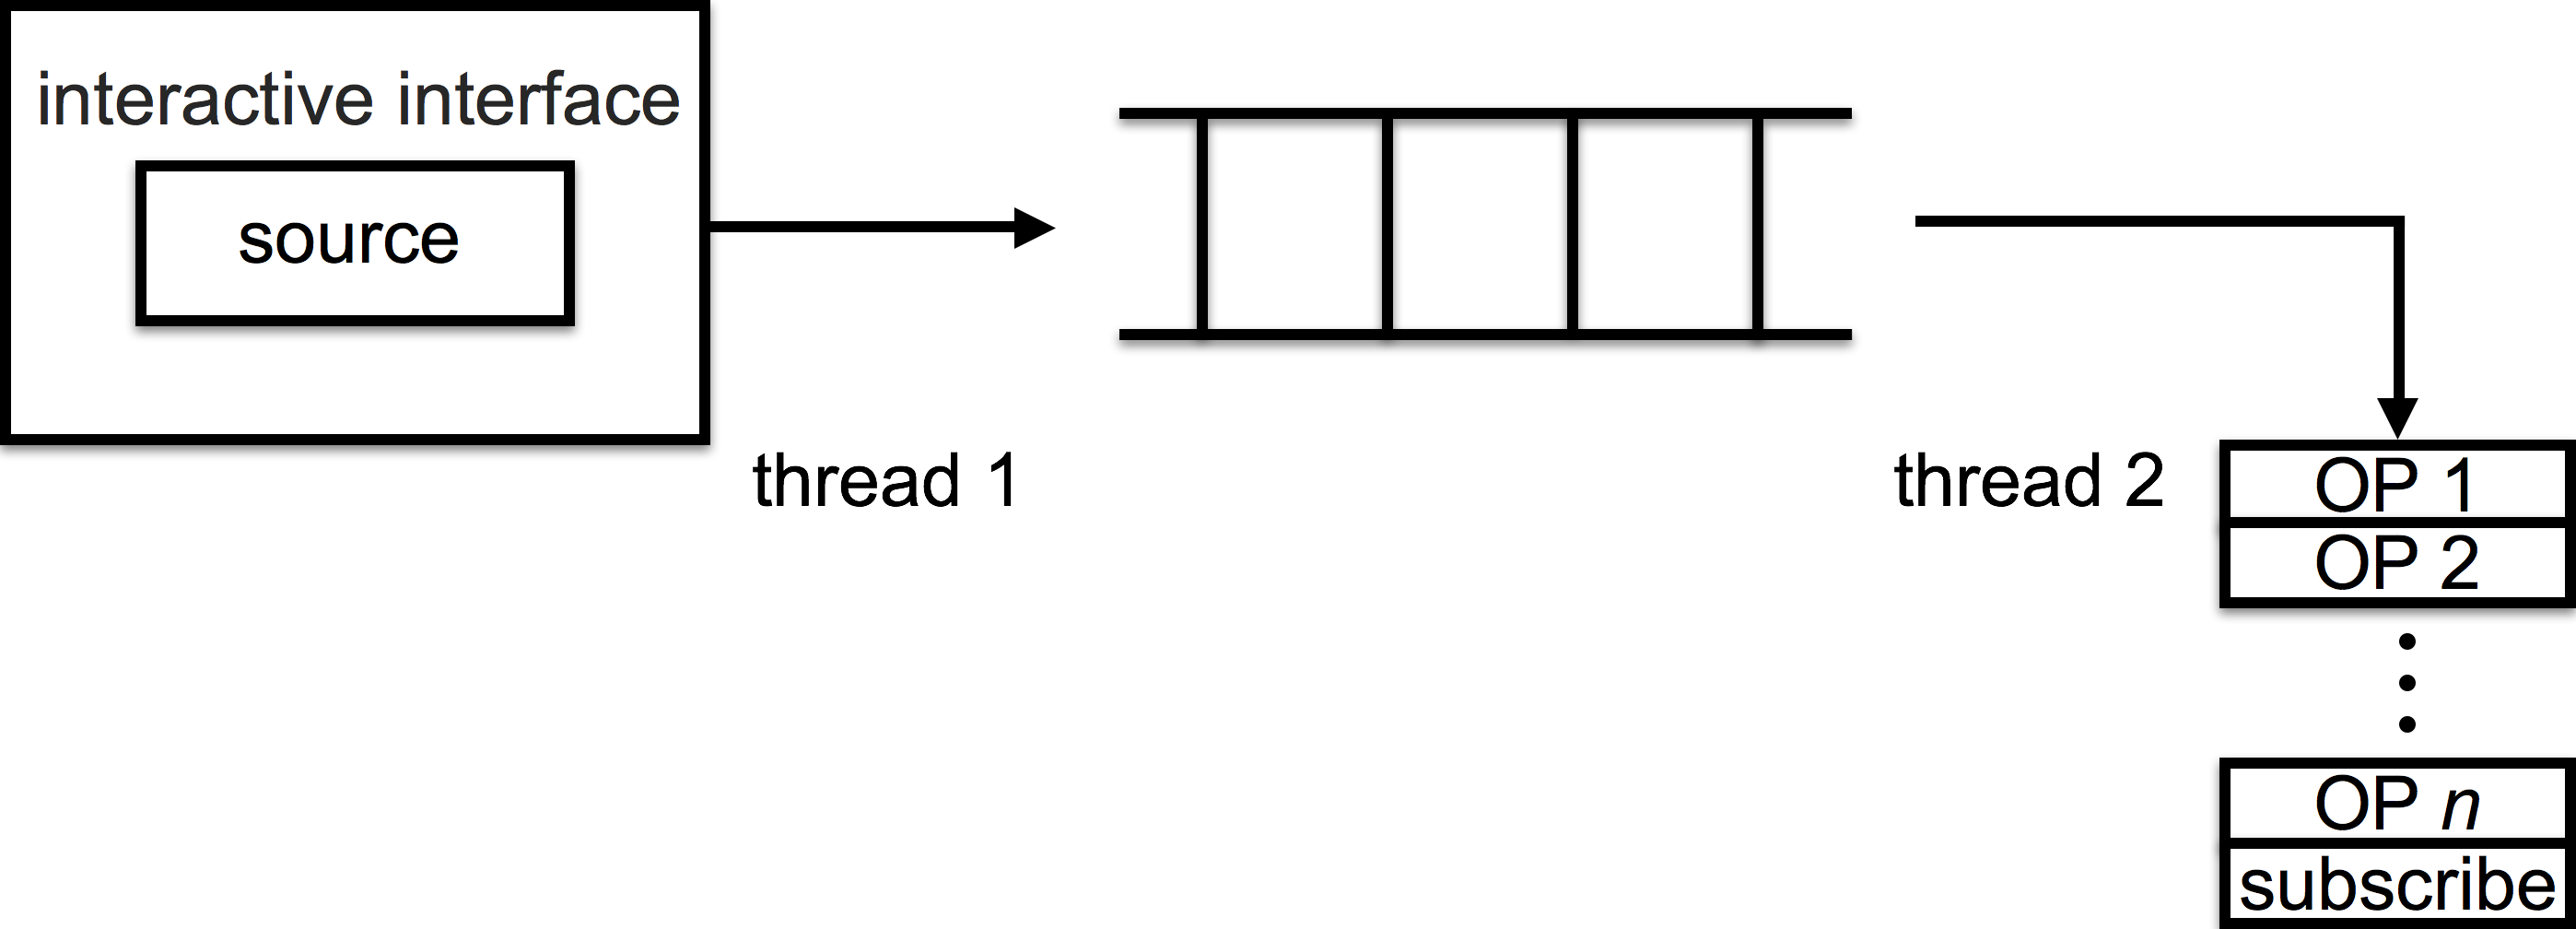
\includegraphics[width=0.63\textwidth]{figures/Approach.png}
	\end{center}
	\caption{Schematic representation of our approach}
	\label{fig:new-approach}
\end{figure}

With this approach we have reduced the problem of overproduction to a problem of controlling the size of a buffer to be as small as possible, without the buffer being exhausted by a fast consuming downstream. A buffer size that is too small can lead to a needless delay in consuming the data, whereas a too large buffer size is not desirable as well, given that we want to spend as little resources as possible. The complicating factor here is that it is unknown at all times how long it will take for the source to produce a next element.

In order to overcome this unknown factor, control the size of the buffer and only request new elements from the source when needed, we will use a well-known technique from mechanical and electrical engineering called \textit{feedback control}. Since this is a technique that is unfortunately not as well-known in computer science and software engineering as it is in other parts of science and engineering, we will introduce this technique in the upcoming chapters, develop an API to work with this technique in general and present the rest of our solution to the overproduction problem after that.

Obviously RxJava in its current stage cannot be used to implement this solution, as it already has a backpressure implementation. Therefore we will use the RxMobile \cite{RxMobile} reference implementation which was recently written in Scala by Erik Meijer as a basic API for reactive programming and build our approach on top of that without the need of rewriting any existing code.
